\documentclass{article}

\usepackage[T1]{fontenc}
\usepackage[utf8]{inputenc}
\usepackage[english]{babel}

\usepackage{geometry}
% \usepackage[showframe]{geometry}
\geometry{a4paper, top=3cm, bottom=3cm, left=2cm, right=2cm, heightrounded}
\usepackage{cancel}
\usepackage{multirow,multicol}
\usepackage[table, x11names]{xcolor}
\usepackage{booktabs}
\usepackage{tabularx}
\usepackage{graphicx}

\usepackage{hyperref}
\hypersetup{
    colorlinks=true,
    linkcolor=blue,
    filecolor=magenta,
    urlcolor=cyan,
    }

\begin{document}

\title{
   \Huge
   2024 \textsc{Kratos Multiphysics\\Workshop @ UNIPD}
}
\author{
   \small
   \begin{tabular}{rl}
      \textsc{Antonia Larese} & \textit{University of Padova (Italy)} \\
      \textsc{Rubén Zorrilla Martínez} & \textit{UPC/CIMNE (Spain)} \\
      \textsc{Carlos Roig} & \textit{CIMNE (Spain)} \\
      \textsc{Suneth Warnakulasuriya} & \textit{Technische Universitat Braunschweig (Germany)} \\
      \textsc{Nicol\`o Crescenzio} & \textit{University of Padova (Italy)}
   \end{tabular}
}
\date{\textsc{November} 6-8, 2024}
\maketitle

\renewcommand{\arraystretch}{1.5}

\section*{\centering\textsc{Kratos Workshop Day 1 -- November 6th, 2024}}

\begin{table}[h]\centering
   \begin{tabularx}{0.85\textwidth}{r|X}
      \toprule%\rule{0mm}{5mm}
      % {\large Time} & {\large Description} \\%[1ex]
      % \midrule%\rule{0mm}{5mm}
      14:00 - 14:30 & Welcome \\%[1ex]
      \midrule%\rule{0mm}{5mm}
                    & {\large \textbf{Introduction to Kratos}} \\%[1ex]
      14:30 - 15:15 & Kratos. Why? What? How? An Historical Perspective \textit{(Riccardo Rossi)}\\%[1ex]
      15:15 - 16:00 & Kratos: an Overview \textit{(Pooyan Dadvand)}\\%[1ex]
      \midrule%\rule{0mm}{5mm}
      \rowcolor{SeaGreen3!5!} 16:00 - 16:30 & Coffee Break \\%[1ex]
      \midrule%\rule{0mm}{5mm}
                    & {\large \textbf{Kratos 4 Industry}} \\%[1ex]
      16:30 - 17:00 & Collaboration with Industry in Germany \textit{(Suneth Warnakulasuriya)}\\%[1ex]
      17:00 - 18:00 & Deltares \textit{(Jonathan Nuttall)}\\%[1ex]
      18:00 - 18:30 & Altair \textit{(Pooyan Dadvand)}\\%[1ex]
      \bottomrule
   \end{tabularx}
\end{table}

\newpage
\section*{\centering \textsc{Kratos Workshop Day 2 -- November 7th, 2024}}

\begin{table}[h]\centering
   \begin{tabularx}{0.85\textwidth}{r|X}
      \toprule%\rule{0mm}{5mm}
      % {\large Time} & {\large Description} \\%[1ex]
      % \midrule%\rule{0mm}{5mm}
                    & {\large \textbf{What's New in Kratos? Application Session (1)}} \\%[1ex]
      09:00 - 09:30 & Computational Fluid Dynamics \textit{(Rubén Zorrilla Martínez)}\\%[1ex]
      09:30 - 10:00 & Computational Solid Mechanics \textit{(Suneth Warnakulasuriya)}\\%[1ex]
      10:00 - 10:30 & Reduced Order Models \textit{(Riccardo Rossi)}\\%[1ex]
      \midrule%\rule{0mm}{5mm}
      \rowcolor{SeaGreen3!5!} 10:30 - 11:00 & Coffee Break \\%[1ex]
      \midrule%\rule{0mm}{5mm}
                    & {\large \textbf{What's New in Kratos? Application Session (2)}} \\%[1ex]
      11:00 - 11:30 & Coupling: the CoSimulationApplication \textit{(Rubén Zorrilla Martínez)}\\%[1ex]
      11:30 - 12:00 & Particle Methods: the MPMApplication \textit{(Antonia Larese)}\\%[1ex]
      12:00 - 12:30 & TBD \\%[1ex]
      \midrule%\rule{0mm}{5mm}
      \rowcolor{SeaGreen3!5!} 12:30 - 14:00 & Lunch Break \\%[1ex]
      \midrule%\rule{0mm}{5mm}
                    & {\large \textbf{What's New in Kratos? Application Session (3)}} \\%[1ex]
      14:00 - 15:00 & The GeoMechanicsApplication \textit{(Jonathan Nuttall)}\\%[1ex]
      \midrule%\rule{0mm}{5mm}
                    & {\large \textbf{What's New in Kratos? Core Session}} \\%[1ex]
      15:00 - 16:00 & GUI and FlowGraph, Multistage and Register \textit{(Carlos Roig)}\\%[1ex]
      \midrule%\rule{0mm}{5mm}
      16:00 - 18:00 & Round Table \& Coffee \\%[1ex]
      \bottomrule
   \end{tabularx}
\end{table}

\newpage
\section*{\centering \textsc{Kratos Course -- November 8th, 2024}}

%                     & {\textcolor{blue}{$\bullet$ Downloading Python}} \\[-1.5ex]
% \noindent Highlighted in {\color{blue}blue} there are the hands-on exercises for the audience.
% These exercises will be already solved in a Google Colab workbook.

\begin{table}[h]\centering
   \begin{tabularx}{0.85\textwidth}{r|X}
      \toprule%\rule{0mm}{5mm}
      % {\large Time} & {\large Description} \\%[1ex]
      % \midrule%\rule{0mm}{5mm}
      09:00 - 09:15 & {\large \textbf{Introduction: What is Kratos?}} (Carlos Roig) \\%[1ex]
      \midrule%\rule{0mm}{5mm}
      09:15 - 09:45 & {\large \textbf{Environment Setup and Kratos Installation}} (Carlos Roig) \\%[1ex]
      \midrule%\rule{0mm}{5mm}
      09:45 - 10:00 & {\large \textbf{Installation Troubleshooting}} (Carlos Roig) \\%[1ex]
      \midrule%\rule{0mm}{5mm}
      10:00 - 10:30 & {\large \textbf{Basic I/O}} (Rubén Zorrilla Martínez) \\%[1ex]
      \midrule%\rule{0mm}{5mm}
      \rowcolor{SeaGreen3!5!} 10:30 - 11:00 & Coffee Break \\%[1ex]
      \midrule%\rule{0mm}{5mm}
      11:00 - 11:45 & {\large \textbf{Geometry Management}} (Suneth Warnakulasuriya) \\%[1ex]
      \midrule%\rule{0mm}{5mm}
      11:45 - 12:30 & {\large \textbf{Data Management}} (Riccardo Rossi) \\%[1ex]
      \midrule%\rule{0mm}{5mm}
      \rowcolor{SeaGreen3!5!} 12:30 - 14:00 & Lunch Break \\%[1ex]
      \midrule%\rule{0mm}{5mm}
      14:00 - 14:45 & {\large \textbf{Simulation Loop}} (Rubén Zorrilla Martínez) \\%[1ex]
      \midrule%\rule{0mm}{5mm}
      14:45 - 16:00 & {\large \textbf{Multiphysics \& Multistage}} (Pooyan Dadvand) \\%[1ex]
      \midrule%\rule{0mm}{5mm}
      \rowcolor{SeaGreen3!5!} 16:00 - 16:30 & Coffee Break \\%[1ex]
      \midrule%\rule{0mm}{5mm}
      16:30 - 17:00 & {\large \textbf{Q\&A and Technical Discussions}} \\%[1ex]
      \bottomrule
   \end{tabularx}
\end{table}

\newpage
\section*{\centering \textsc{Workshop Venue}}

\noindent The workshop will be held at the \textit{Department of Mathematics ``Tullio Levi-Civita''} of the University of Padova.\\

\noindent \textbf{\textsc{Building Address:}} \href{https://www.google.com/maps/place/Torre+Archimede,+Via+Trieste,+63,+35121+Padova+PD/@45.4113787,11.8848977,901m/data=!3m2!1e3!4b1!4m6!3m5!1s0x477eda58b44676df:0xfacae5884fca17f5!8m2!3d45.4113787!4d11.8874726!16s\%2Fg\%2F12xqbl_z1?entry=ttu&g_ep=EgoyMDI0MTAwOC4wIKXMDSoASAFQAw\%3D\%3D}{``Torre Archimede'', University of Padova, Via Trieste 63, 35121, Padova (Italy)}.\\

\noindent \textbf{\textsc{Room:}} the building has four entrances, marked by letters \texttt{A}, \texttt{B}, \texttt{C} and \texttt{D}.
The workshop will be held in a room located on \underline{floor $-1$ and accessible only by using the stairs (or the elevator) at entrance \texttt{B}}.

\begin{figure}[h]\centering
   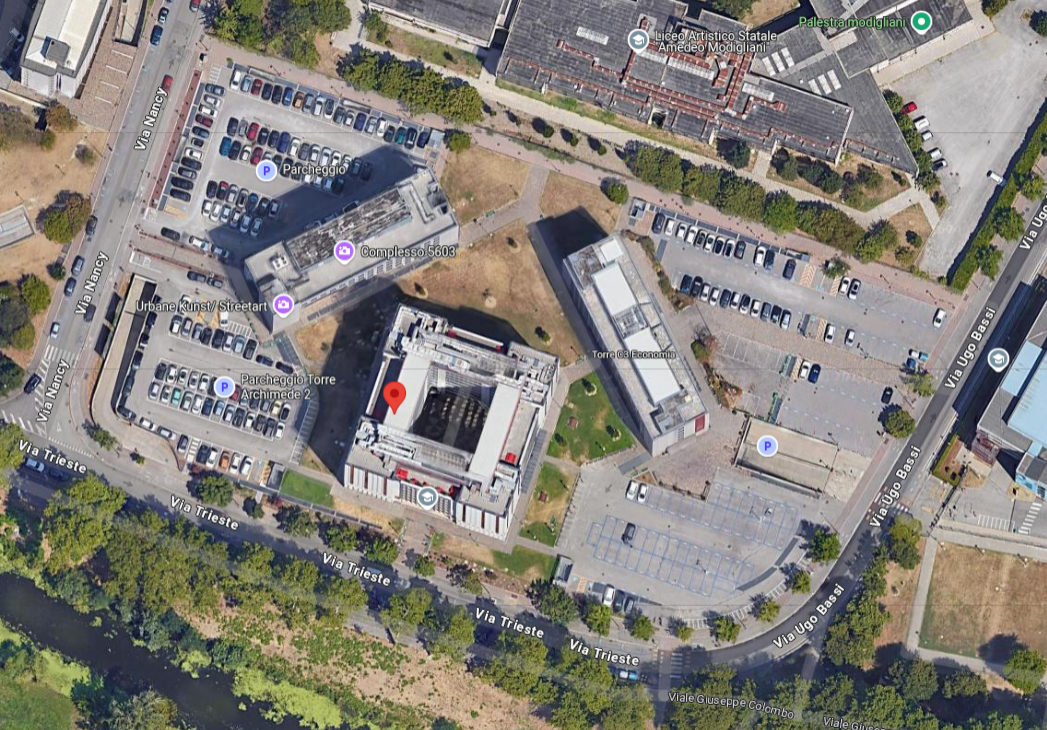
\includegraphics[height=50mm]{figures/google-maps-torre-archimede-1.png}
   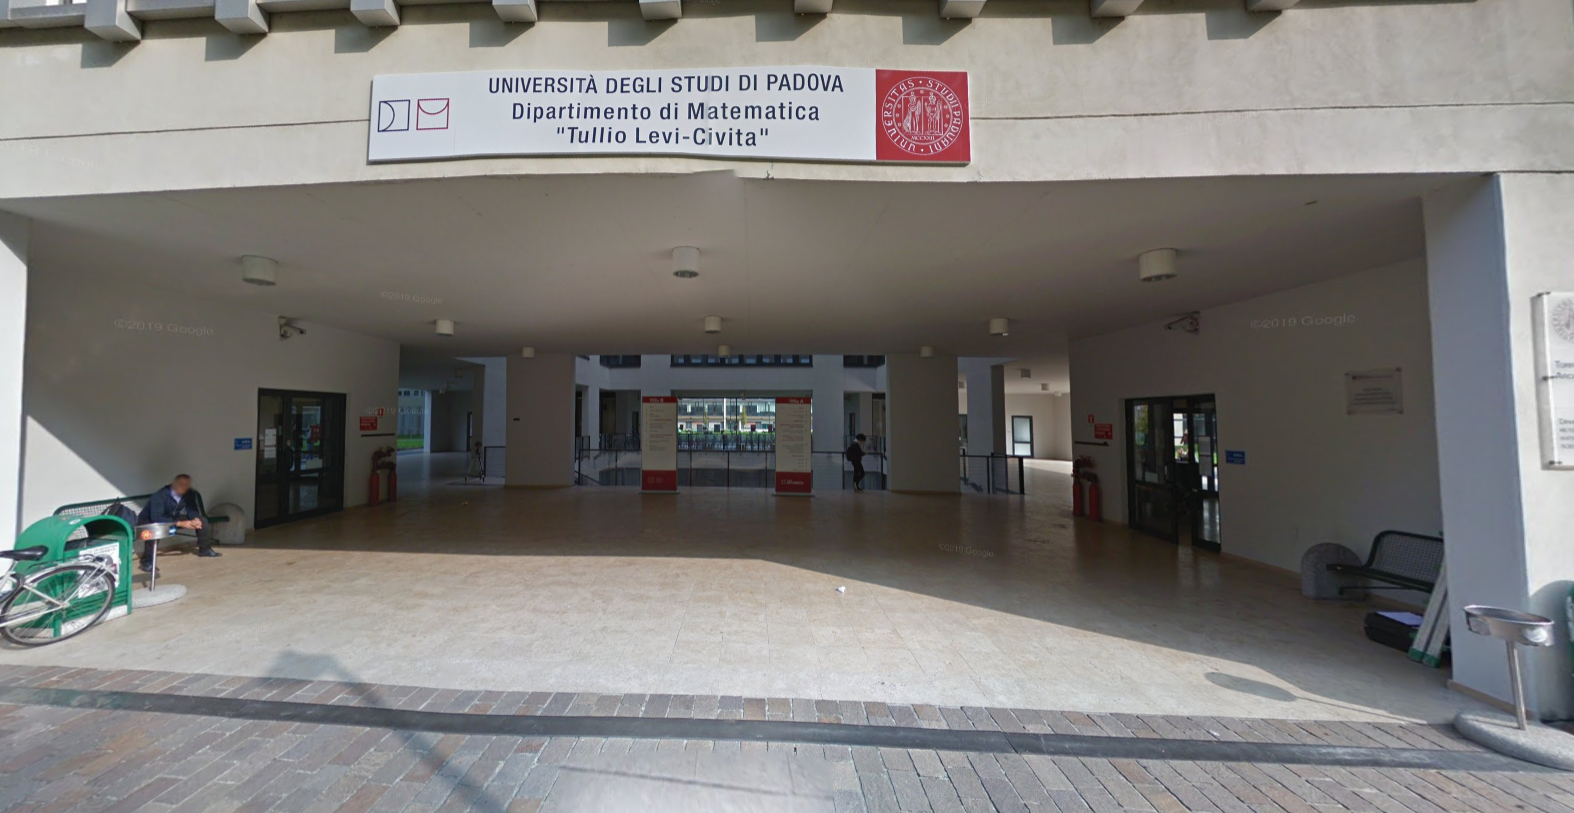
\includegraphics[height=50mm]{figures/google-maps-torre-archimede-2.png}
   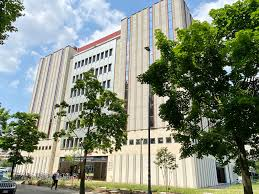
\includegraphics[height=59mm]{figures/torre-archimede-1.jpeg}
   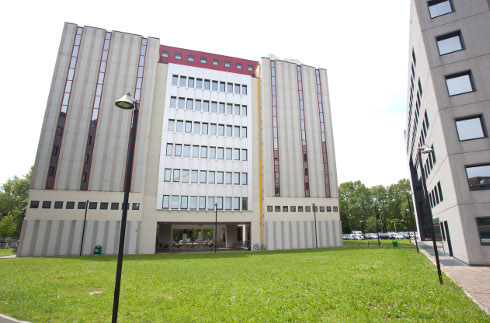
\includegraphics[height=59mm]{figures/torre-archimede-2.jpg}
   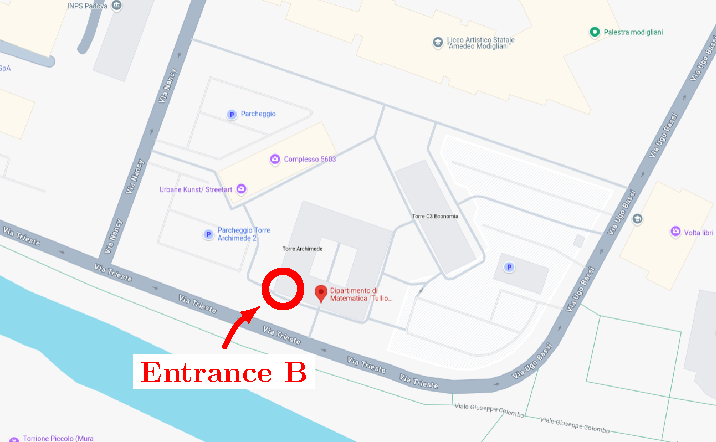
\includegraphics[height=74mm, trim={15mm 0mm 10mm 10mm}, clip]{figures/google-maps-torre-archimede-4.pdf}
   % 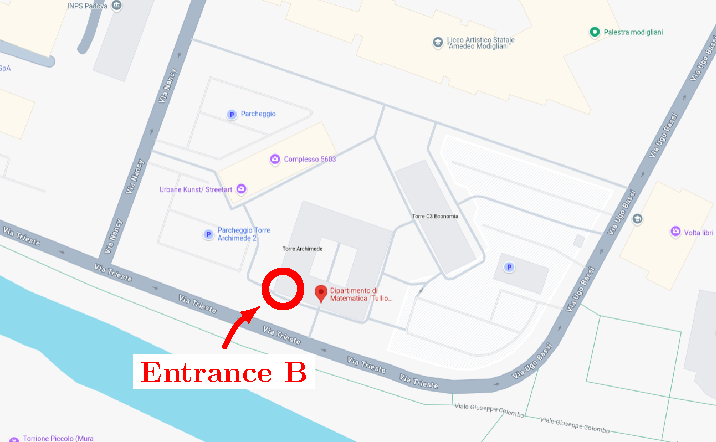
\includegraphics[height=74mm, trim={60mm 0mm 80mm 50mm}, clip]{figures/google-maps-torre-archimede-4.pdf}
\end{figure}


\end{document}
